\documentclass{report}
\usepackage{amsmath}
\usepackage{pgf}
\usepackage{graphicx}
\usepackage{tikz}
\usepackage{pgfplots}

\begin{document}
\title{Sorting Algorithms}
\author{Philip J.Y. Lee}
\maketitle

\chapter{1}
\section{Introduction to Sorting Algorithms}
\subsection{Insertion Sort}
Insertion sort is a kind of sort that...
\subsection{Merge Sort}
Merger sort is a kind of sort that...
\subsection{Heap Sort}
Heap sort is a kind of sort that...
\subsection{Quick Sort}
Quick sort is a kind of sort that...

\chapter{2}
% GRAPHICS
%\usepackage{pgf}
%\usepackage{graphicx}
%\usepackage{tikz}
%\usepackage{pgfplots}
%==========For Failure===========

 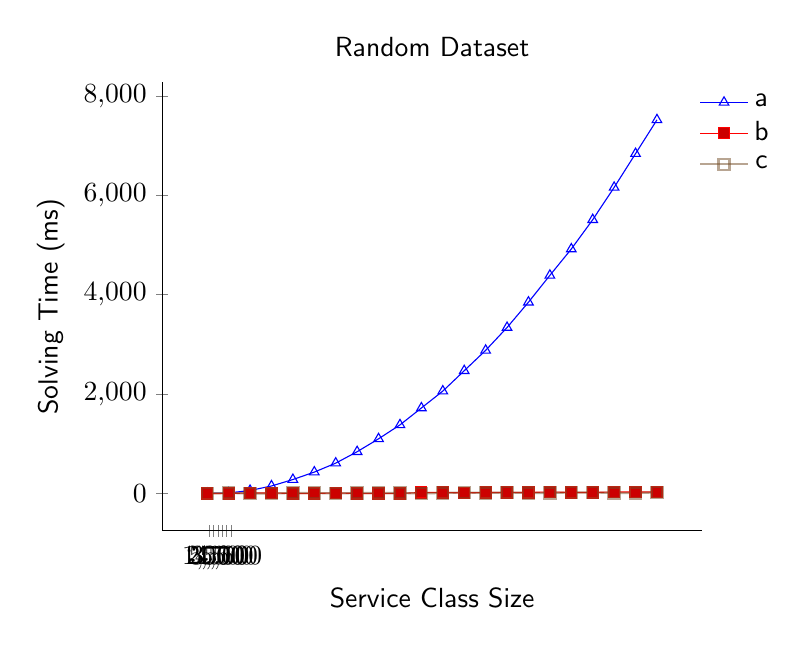
\begin{tikzpicture}[font=\sffamily]
 \begin{axis}[title=Random Dataset,
                              legend pos=outer north east,
                              legend style={draw=none},
                              xtick={500,1500,...,5000}, % new bit
                              scaled ticks=false,
                              log ticks with fixed point={1000 sep=},
                              axis x line=bottom,
                              axis y line=left,
                              axis line style=-,
                              minor tick style={draw=none},
                              enlargelimits,
                              ylabel = Solving Time (ms),
                              xlabel = Service Class Size,
                              every axis legend/.append style={xshift=-10pt}
                              ]
 \addplot+[mark=triangle] plot coordinates{(10, 0.000000) (5000, 10.000000) (10000, 60.000000) (15000, 150.000000) (20000, 280.000000) (25000, 430.000000) (30000, 610.000000) (35000, 840.000000) (40000, 1100.000000) (45000, 1380.000000) (50000, 1720.000000) (55000, 2060.000000) (60000, 2470.000000) (65000, 2880.000000) (70000, 3340.000000) (75000, 3850.000000) (80000, 4390.000000) (85000, 4920.000000) (90000, 5510.000000) (95000, 6160.000000) (100000, 6840.000000) (105000, 7520.000000) };
 \addplot plot coordinates{(10, 0.000000) (5000, 0.000000) (10000, 10.000000) (15000, 10.000000) (20000, 0.000000) (25000, 0.000000) (30000, 10.000000) (35000, 0.000000) (40000, 0.000000) (45000, 0.000000) (50000, 20.000000) (55000, 20.000000) (60000, 10.000000) (65000, 20.000000) (70000, 20.000000) (75000, 20.000000) (80000, 30.000000) (85000, 20.000000) (90000, 20.000000) (95000, 30.000000) (100000, 30.000000) (105000, 30.000000) };
 \addplot+[draw opacity=0.5, thick, mark=square] plot coordinates{(10, 0.000000) (5000, 10.000000) (10000, 0.000000) (15000, 0.000000) (20000, 10.000000) (25000, 10.000000) (30000, 0.000000) (35000, 10.000000) (40000, 10.000000) (45000, 10.000000) (50000, 0.000000) (55000, 10.000000) (60000, 20.000000) (65000, 10.000000) (70000, 20.000000) (75000, 10.000000) (80000, 10.000000) (85000, 20.000000) (90000, 20.000000) (95000, 10.000000) (100000, 10.000000) (105000, 20.000000) };
 \legend{a,b,c}
 \end{axis}
 \end{tikzpicture}

 %==========For Failure===========



\end{document}
